% Point to the main file
\documentclass[../../Main.tex]{subfiles}

% ========== Start the document ==========
\begin{document}

\section{Section 2.2 - Set Operations}

Let's consider a venn diagram which is a way of visualizing sets

Let $U$ represent the \yellowbox{universal set}

\begin{definition}[Intersection]
    Elements that are in \textbf{both} \mathset{A} and \mathset{B} is called the \yellowbox{intersection} of \mathset{A} and \mathset{B}
    $$ \mathset{A} \cap \mathset{B} $$

    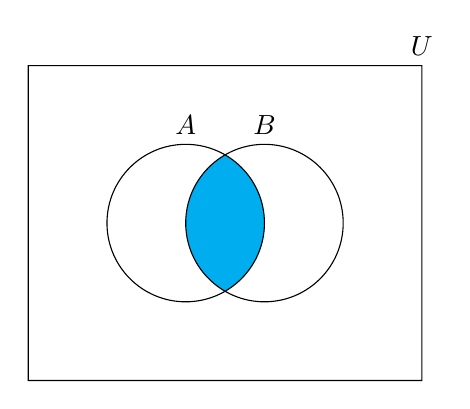
\begin{tikzpicture}[fill=cyan]

    \scope

    \clip (-2,-2) rectangle (2,2)
        (1,0) circle (1)
        (0,0) circle (1);
    \fill (0,0) circle (1);

    \endscope

    % outline
    \draw (0,0) circle (1) (0,1)  node [text=black,above] {$A$}
        (1,0) circle (1) (1,1)  node [text=black,above] {$B$}
        (-2,-2) rectangle (3,2) node [text=black,above] {$U$};
    \end{tikzpicture}
\end{definition}

\begin{definition}[Union]
    Elements that are in \textbf{either} \mathset{A} or \mathset{B} is called the \yellowbox{union} of \mathset{A} and \mathset{B}
    $$ \mathset{A} \cup \mathset{B} $$

    Also

    $$ | \mathset{A} \cup \mathset{B} | = | \mathset{A} | + | \mathset{B} | - | \mathset{A} \cap \mathset{B} | $$

    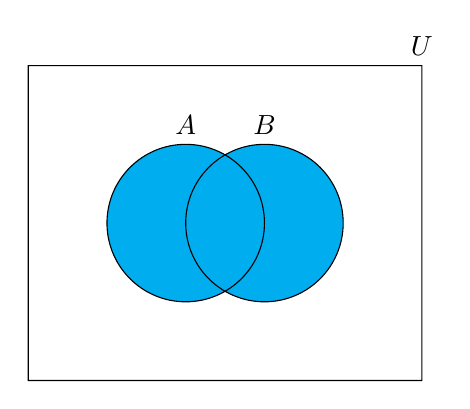
\begin{tikzpicture}[fill=cyan]
    % left hand
    \scope
    \clip (-2,-2) rectangle (2,2)
        (1,0) circle (1);
    \fill (0,0) circle (1);
    \endscope
    % right hand
    \scope
    \clip (-2,-2) rectangle (2,2);
    \fill (1,0) circle (1);
    \endscope
    % outline
    \draw (0,0) circle (1) (0,1)  node [text=black,above] {$A$}
        (1,0) circle (1) (1,1)  node [text=black,above] {$B$}
        (-2,-2) rectangle (3,2) node [text=black,above] {$U$};
    \end{tikzpicture}
\end{definition}

\begin{definition}[Compliment]
    Elements that just aren't in \mathset{A} is called the \yellowbox{compliment} of \mathset{A}
    $$ \overline{\mathset{A}} $$

    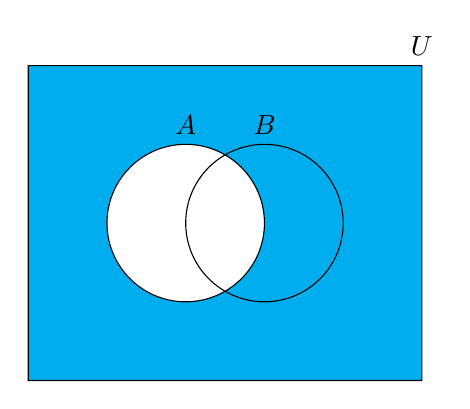
\begin{tikzpicture}[fill=cyan]
    % left hand
    \scope

    % \clip (1,0) circle (1);
    \fill (0,0) circle (1)
        (-2,-2) rectangle (3,2);
    \endscope
    % right hand
    \scope
    \clip (-2,-2) rectangle (3,2)
        (0,0) circle (1);
    \fill (1,0) circle (1);
    \endscope
    % outline
    \draw (0,0) circle (1) (0,1)  node [text=black,above] {$A$}
        (1,0) circle (1) (1,1)  node [text=black,above] {$B$}
        (-2,-2) rectangle (3,2) node [text=black,above] {$U$};
    \end{tikzpicture}
\end{definition}

\begin{definition}[Difference]
    Elements in \mathset{B} but not in \mathset{A} is called the \yellowbox{difference}
    $$ \mathset{B} - \mathset{A} $$

    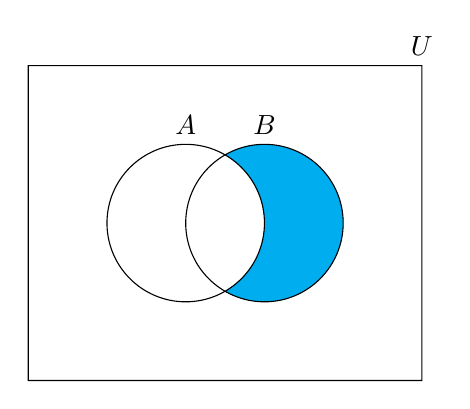
\begin{tikzpicture}[fill=cyan]
    % left hand
    \scope

    \clip (1,0) circle (1);
    \fill (0,0) circle (1)
        (-2,-2) rectangle (3,2);
    \endscope
    % right hand
    \scope
    \clip (-2,-2) rectangle (3,2)
        (0,0) circle (1);
    \fill (1,0) circle (1);
    \endscope
    % outline
    \draw (0,0) circle (1) (0,1)  node [text=black,above] {$A$}
        (1,0) circle (1) (1,1)  node [text=black,above] {$B$}
        (-2,-2) rectangle (3,2) node [text=black,above] {$U$};
    \end{tikzpicture}
\end{definition}

With sets, we have 3 operations:

\begin{enumerate}
    \item Compliment $\overline{\mathset{A}}$ \; (analogous to $\neg$)

    \item Union $\mathset{A} \cup \mathset{B}$ \; (analogous to $\lor$)
    
    \item Intersection $\mathset{A} \cap \mathset{B}$ \; (analogous to $\land$)
\end{enumerate}

\begin{example}
    Let 
    
    \begin{align*}
        \mathset{U} &= \{ x \in \setZ \mid 0 \leq x \leq 20 \} \\
        \mathset{A} &= \{ x \in \mathset{U} \mid x \text{ is even} \} \\
        \mathset{B} &= \{ x \in \mathset{U} \mid x \text{ is divisible by 3} \} \\
    \end{align*}

    Determine the following

    \begin{enumerate}
        \item $\mathset{A} = \{ 0, 2, 4, 6, 8, 10, 12, 14, 16, 18, 20 \}$
        \item $\mathset{B} = \{ 0, 3, 6, 9, 12, 15, 18 \}$
        \item $\mathset{A} \cap \mathset{B} = \{ 0, 6, 12, 18 \}$ \; (what they have in common)
        \item $\mathset{A} \cup \mathset{B} = \{ 0, 2, 3, 4, 6, 8, 9, 10, 12, 14, 15, 16, 18, 20 \}$ \; (whats in either one)
        \item $\overline{\mathset{A}} = \{ 1, 3, 5, 7, 9, 11, 13, 15, 17, 19 \}$ \; (whats not in A)
        \item $\mathset{B} - \mathset{A} = \{ 3, 9, 15 \}$ \; (what's in B thats not in A)
        \item $| \mathset{A} | = 11$ \; (number of elements in $\mathset{A}$)
        \item $| \mathset{B} | = 7$ \; (number of elements in $\mathset{B}$)
        \item $| \mathset{A} \cup \mathset{B} | = 14$
        \item $| \mathset{A} \cap \mathset{B} | = 4$ (number of elements that $\mathset{A}$ and $\mathset{B}$ have in common)
        \item $| \mathset{A} | + | \mathset{B} | - | \mathset{A} \cap \mathset{B} | = 11 + 7 - 4 = 14 = | \mathset{A} \cup \mathset{B} |$
    \end{enumerate}
\end{example}

But how do these operations interact together?

\begin{example}
    \;
    \begin{itemize}
        \item $\overline{\mathset{A} \cup \mathset{B}}$
        
            Red = $\mathset{A} \cup \mathset{B}$
            \\
            Blue = $\overline{\mathset{A} \cup \mathset{B}}$

            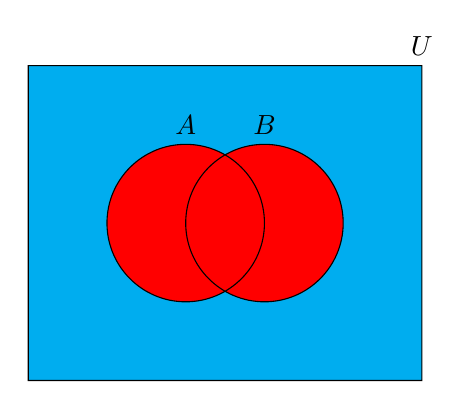
\begin{tikzpicture}%[fill=red]

            % A is (0,0) circle (1)
            % B is (1,0) circle (1)
            % U is (-2,-2) rectangle (3,2)

            \scope

            \clip (-2,-2) rectangle (3,2) 
                (0,0) circle (1)
                (1,0) circle (1);

            \fill[cyan] (-2,-2) rectangle (3,2);

            \endscope

            % left hand
            \scope

            % \clip (1,0) circle (1);
            \fill[red] (0,0) circle (1)
                (1,0) circle (1);
                % (-2,-2) rectangle (3,2);

            \endscope

            % outline
            \draw (0,0) circle (1) (0,1)  node [text=black,above] {$A$}
                (1,0) circle (1) (1,1)  node [text=black,above] {$B$}
                (-2,-2) rectangle (3,2) node [text=black,above] {$U$};
            \end{tikzpicture}

        \item $\overline{\mathset{A}} \cap \overline{\mathset{B}}$
        
            Red = $\overline{\mathset{A}}$
            \\
            Blue = $\overline{\mathset{B}}$
            \\
            Purple = $\overline{\mathset{A}} \cap \overline{\mathset{B}}$

            % A is (0,0) circle (1)
            % B is (1,0) circle (1)
            % U is (-2,-2) rectangle (3,2)

            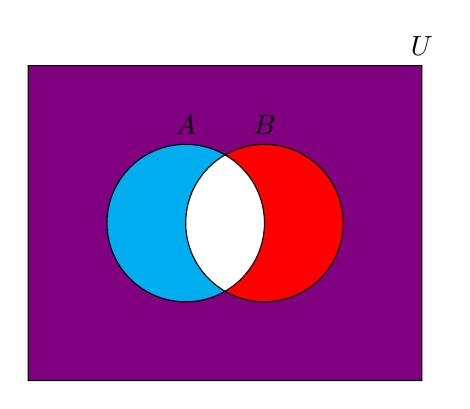
\begin{tikzpicture}%[fill=cyan]
                % left hand
                \scope

                % \clip (1,0) circle (1);
                \fill[violet] (0,0) circle (1)
                    (-2,-2) rectangle (3,2);
                \endscope
                % right hand
                \scope
                \clip (-2,-2) rectangle (3,2)
                    (0,0) circle (1);
                \fill[red] (1,0) circle (1);
                \endscope

                \scope
                \clip (-2,-2) rectangle (3,2)
                    (1,0) circle (1);
                \fill[cyan] (0,0) circle (1);
                \endscope
                % outline
                \draw (0,0) circle (1) (0,1)  node [text=black,above] {$A$}
                    (1,0) circle (1) (1,1)  node [text=black,above] {$B$}
                    (-2,-2) rectangle (3,2) node [text=black,above] {$U$};
            \end{tikzpicture}

        $$\therefore \overline{\mathset{A} \cup \mathset{B}} = \overline{\mathset{A}} \cap \overline{\mathset{B}}$$
    \end{itemize}
\end{example}

\begin{enumerate}
    \item \textbf{DeMorgan's Laws}
    \begin{itemize}
        \item $\overline{\mathset{A} \cup \mathset{B}} = \overline{\mathset{A}} \cap \overline{\mathset{B}}$
        \item $\overline{\mathset{A} \cap \mathset{B}} = \overline{\mathset{A}} \cup \overline{\mathset{B}}$
    \end{itemize}

    \item \textbf{Distributive Laws}
    \begin{itemize}
        \item $\mathset{A} \cap (\mathset{B} \cup \mathset{C}) = (\mathset{A} \cap \mathset{B}) \cup (\mathset{A} \cap \mathset{C})$
        \item $\mathset{A} \cup (\mathset{B} \cap \mathset{C}) = (\mathset{A} \cup \mathset{B}) \cap (\mathset{A} \cup \mathset{C})$
    \end{itemize}

    \item \textbf{Complementation Law}
    \begin{itemize}
        \item $\overline{\overline{\mathset{A}}} = \mathset{A}$
    \end{itemize}

    \item \textbf{Communative Law}
    \begin{itemize}
        \item $\mathset{A} \cup \mathset{B} = \mathset{B} \cup \mathset{A}$
        \item $\mathset{A} \cap \mathset{B} = \mathset{B} \cap \mathset{A}$
    \end{itemize}
   
\end{enumerate}

% ========== End the document ==========
\end{document}